\section{Auswertung}
\label{sec:Auswertung}

\subsection{Bestimmung der Schallgeschwindigkeit}

  Der Acrylblock hat die Maße $ \SI{149.3}{\milli\metre} \times \SI{79.6}{\milli\metre} \times \SI{41.7}{\milli\metre}$, welche mit einer Schieblehre gemessen wurden. 
  Mit dem Ultraschallechoskop werden im Impuls-Echo-Verfahren die Störstellen einmal von der Oberseite, also der Seite, wo die Stellen 1 und 2 oben sind,
  und einmal von der Unterseite gemessen; die Messpunkte bestehen aus Tupel von Zeit und Amplitude.
  Zusätzlich werden die Abstände der Störstellen zur jeweiligen Außenkante mit einer Schieblehre ermittelt. In der \autoref{tab:acrylblock} sind die Messdaten 
  zu finden. 

  \begin{table} 
    \centering
    \caption{Die Werte von den Messungen des Acrylblockes mit Störstellen.}
    \label{tab:acrylblock}
    \begin{tabular}{S[table-format=2] S[table-format=2.1] S[table-format=1.3] S[table-format=2.1] S[table-format=2.1] S[table-format=1.3] S[table-format=2.1]}
      \toprule
      & \multicolumn{3}{c}{Oberseite} & \multicolumn{3}{c}{Unterseite}\\
      \cmidrule(lr){2-4} \cmidrule(lr){5-7}
      Nr & $t \mathbin{/} \si{\micro\second}$ & $ A \mathbin{/} \si{\volt}$ & $ s \mathbin{/} \si{\milli\metre}$ & $t \mathbin{/} \si{\micro\second}$ & $ A \mathbin{/} \si{\volt}$ & $ s \mathbin{/} \si{\milli\metre}$ \\
      \midrule
      1   & 15.2   & 0.134   & 19.2  & 44.0   &  0.025  & 60.4  \\
      2   & 13.9   & 0.118   & 17.5  & 45.1   &  0.017  & 62.1  \\
      3   & 45.1   & 0.039   & 60.2  & 10.7   &  0.305  & 13.4  \\
      4   & 39.6   & 0.025   & 52.9  & 16.8   &  0.188  & 21.8  \\
      5   & 34.1   & 0.031   & 45.3  & 23.0   &  0.050  & 30.3  \\
      6   & 28.6   & 0.056   & 37.1  & 29.1   &  0.062  & 38.6  \\
      7   & 22.9   & 0.090   & 30.3  & 35.0   &  0.045  & 46.6  \\
      8   & 17.0   & 0.132   & 22.3  & 40.9   &  0.045  & 54.7  \\
      9   & 11.2   & 0.199   & 13.8  & 46.6   &  0.022  & 62.7  \\
      10  & 5.4    & 0.303   &  6.8  &        &         & 72.8  \\
      11  & 40.6   & 0.045   & 55.9  & 12.2   &  0.342  & 15.4  \\
      \bottomrule
    \end{tabular}
  \end{table}

  \noindent Es ist zu sehen, dass die Störstelle 10 von der Unterseite nicht durch das Ultraschallechoskop zu messen ist, da diese Stelle komplett durch die 
  Störstelle 11 abgedeckt ist. Da die Stelle 11 einen größeren Durchmesser hat, ist sie von der Oberseite dennoch zu bestimmen. 

  \begin{figure}[H]
    \centering
    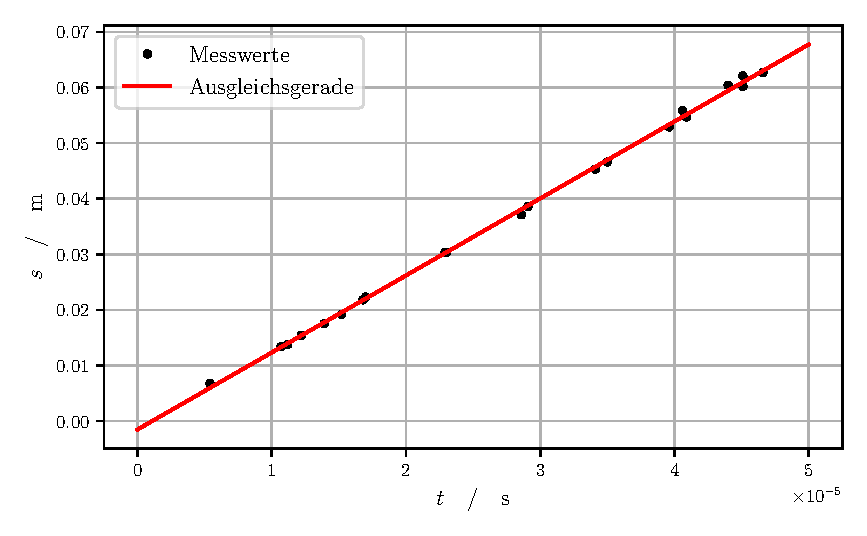
\includegraphics[width=\textwidth]{build/schallgeschwindigkeit.pdf}
    \caption{Die aufgenommenen Werte geplottet inclusive einer Ausgleichsgerade.}
    \label{fig:schallgeschwindigkeit}    
  \end{figure}

  \noindent In der \autoref{fig:schallgeschwindigkeit} sind die Daten aus der \autoref{tab:acrylblock} in einem $t$-$s$-Diagramm aufgetragen. Zusätzlich 
  ist eine Ausgleichsrechnung der Form $ s = a \cdot t + b $ geplottet. Die Parameter ergeben sich zu:
  \begin{align*}
    a = \SI{1385.33(997)}{\metre\per\second}\\
    b = \SI{-0.0015(3)}{\metre}
  \end{align*}
  Durch Vergleich mit der Formel \eqref{eqn:schallgeschw} lässt sich die Schallgeschwindigkeit in Acryl errechnen:
  \begin{equation*}
    c = 2 \cdot a = \SI{2771(20)}{\metre\per\second}
  \end{equation*}


\subsection{Bestimmung des Absoprtionskoeffizienten}

  Nun werden die Werte der Amplitude $A$ aus der \autoref{tab:acrylblock} in Abhängigkeit von der Entfernung zur Außenkante aufgetragen. Für die Strecke 
  wird im folgenden der Ausdruck $ s(t) = c \cdot t $ benutzt. Dies beschreibt die Strecke, die die Schallwelle zurücklegt, bis sie vom dem Ultraschallechoskop
  wieder aufgenommen wird. Der Plot ist in der \autoref{fig:absorptionskoeff} zu finden. 

  \begin{figure}[H]
    \centering
    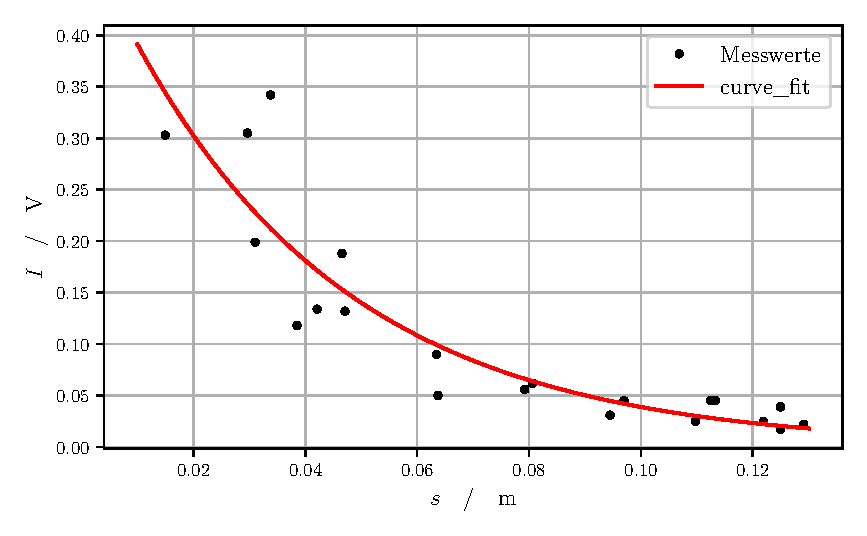
\includegraphics[width=\textwidth]{build/absorptionskoeff.pdf}
    \caption{Die Amplitude aufgetragen gegen die im Acrylblock zurückgelegte Strecke.}
    \label{fig:absorptionskoeff}
  \end{figure}

  \noindent In die \autoref{fig:absorptionskoeff} ist außerdem eine Ausgleichsrechnung der Form $ I = I_0 \cdot \symup{e}^{-\alpha \cdot x} $ eingetragen. 
  Die Parameter dafür ergeben sich zu: 
  \begin{align*}
    I_0 = \SI{0.5054(724)}{\volt}\\
    \alpha = \SI{25.6531(37636)}{\per\metre}
  \end{align*}
  Der Absorptionskoeffizient wird mit $\alpha$ beschrieben.


\subsection{Bestimmung der Abstände im Auge}

  Abschließend wird das Augenmodell mit dem Ultraschallechoskop untersucht. In dem Foto \ref{fig:augenpeaks} sind drei Peaks zu sehen. Es wird vermutet, dass der 
  erste Peak die Reflektion an der Iris, der Zweite die Reflektion an der Linse und der dritte Peak die Reflektion an der Retina beschreibt. Die Zeiten wurden 
  abgelesen zu:
  \begin{align*}
    t_1 &= \SI{11.3}{\micro\second} \\
    t_{\text{Linse}} &= \SI{17.4}{\micro\second}\\
    t_{\text{Retina}} &= \SI{24.6}{\micro\second}
  \end{align*}

  \noindent Mit den Schallgeschwindigkeiten für die Glaskörperflüssigkeit und das Linsenmaterial des Augenmodells, $c_{\text{Gk}} = \SI{1410}{\metre\per\second}$ und
  $c_{\text{L}} = \SI{2500}{\metre\per\second}$ nach \cite{anleitung}, lassen sich nun die Abstände im Augenmodell bestimmen. Sie lauten:

  \begin{align*}
    s_{\text{Iris}}   &= \frac{c_{\text{Gk}} \cdot t_1}{2}                                              &= \SI{7.9665}{\milli\metre} \\
    s_{text{Linse}}   &= \frac{(t_2 - t_1) \cdot c_{\text{L}}}{2} + s_{\text{Iris}}                     &= \SI{15.5915}{\milli\metre} \\
    s_{text{Retina}}  &= \frac{(t_3 - t_2) \cdot c_{\text{Gk}}}{2} + s_{\text{Iris}} + s_{\text{Linse}} &= \SI{20.6675}{\milli\metre}.
  \end{align*}

  \begin{figure}[H]
    \centering
    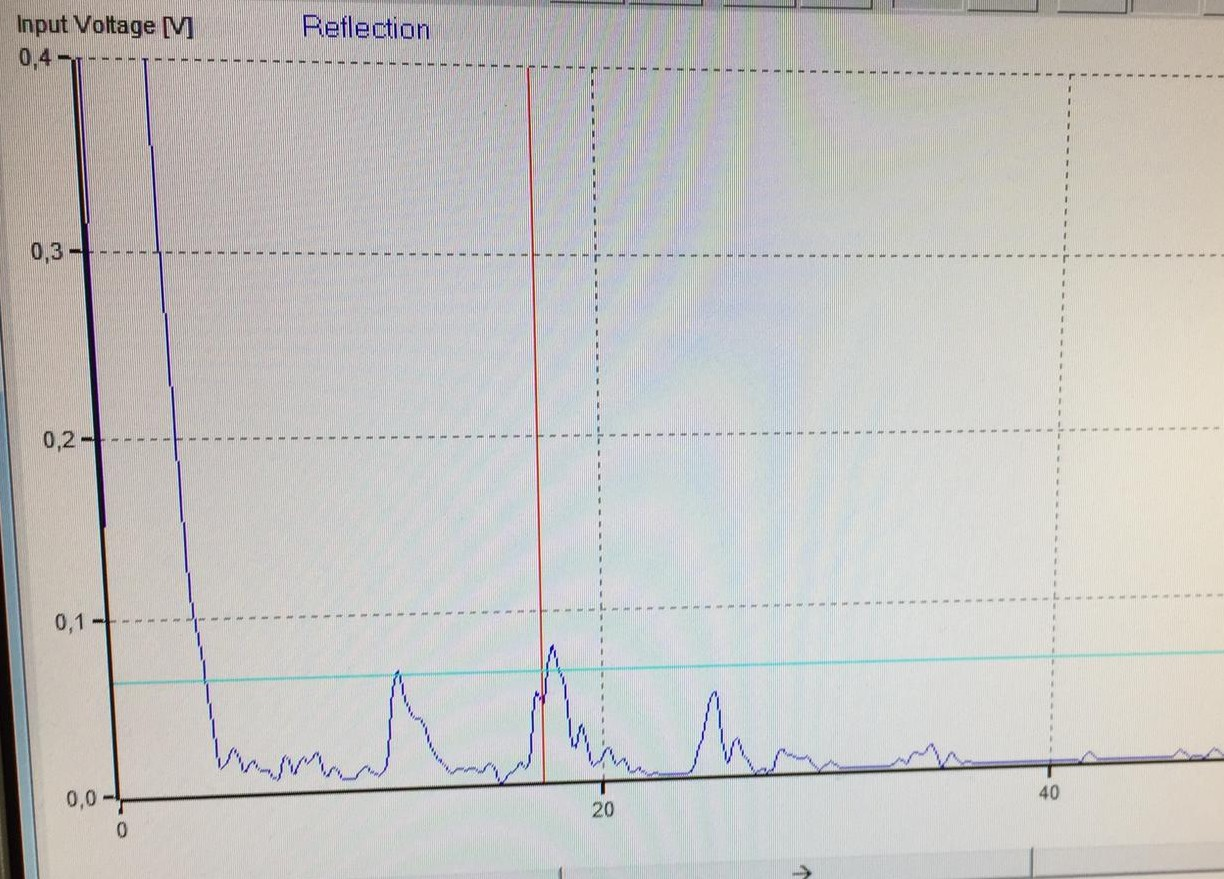
\includegraphics[width=\textwidth]{content/foto_messwerte_auge.jpeg}
    \caption{Das Foto von den aufgenommenen Peaks beim Messen des Augenmodells.}
    \label{fig:augenpeaks}
  \end{figure}